\ifx\wholebook\relax \else
% ------------------------ 

\documentclass{article}
%------------------- Other types of document example ------------------------
%
%\documentclass[twocolumn]{IEEEtran-new}
%\documentclass[12pt,twoside,draft]{IEEEtran}
%\documentstyle[9pt,twocolumn,technote,twoside]{IEEEtran}
%
%-----------------------------------------------------------------------------
%%
% loading packages
%
\newif\ifpdf
\ifx\pdfoutput\undefined % We're not running pdftex
  \pdffalse
\else
  \pdftrue
\fi
%
%
\ifpdf
  \RequirePackage[pdftex,%
            CJKbookmarks,%
       bookmarksnumbered,%
              colorlinks,%
          linkcolor=blue,%
              hyperindex,%
        plainpages=false,%
       pdfstartview=FitH]{hyperref}
\else
  \RequirePackage[dvipdfm,%
             CJKbookmarks,%
        bookmarksnumbered,%
               colorlinks,%
           linkcolor=blue,%
               hyperindex,%
         plainpages=false,%
        pdfstartview=FitH]{hyperref}
  \AtBeginDvi{\special{pdf:tounicode GBK-EUC-UCS2}} % GBK -> Unicode
\fi
\usepackage{hyperref}

% other packages
%-----------------------------------------------------------------------------
\usepackage{graphicx, color}
\usepackage{CJK}
%
% for programming 
%
\usepackage{verbatim}
\usepackage{listings}


\lstdefinelanguage{Smalltalk}{
  morekeywords={self,super,true,false,nil,thisContext}, % This is overkill
  morestring=[d]',
  morecomment=[s]{"}{"},
  alsoletter={\#:},
  escapechar={!},
  literate=
    {BANG}{!}1
    {UNDERSCORE}{\_}1
    {\\st}{Smalltalk}9 % convenience -- in case \st occurs in code
    % {'}{{\textquotesingle}}1 % replaced by upquote=true in \lstset
    {_}{{$\leftarrow$}}1
    {>>>}{{\sep}}1
    {^}{{$\uparrow$}}1
    {~}{{$\sim$}}1
    {-}{{\sf -\hspace{-0.13em}-}}1  % the goal is to make - the same width as +
    %{+}{\raisebox{0.08ex}{+}}1		% and to raise + off the baseline to match -
    {-->}{{\quad$\longrightarrow$\quad}}3
	, % Don't forget the comma at the end!
  tabsize=2
}[keywords,comments,strings]

\lstloadlanguages{C++, Lisp, Smalltalk}

% ======================================================================

\def\BibTeX{{\rm B\kern-.05em{\sc i\kern-.025em b}\kern-.08em
    T\kern-.1667em\lower.7ex\hbox{E}\kern-.125emX}}

\newtheorem{theorem}{Theorem}

%
% mathematics
%
\newcommand{\be}{\begin{equation}}
\newcommand{\ee}{\end{equation}}
\newcommand{\bmat}[1]{\left( \begin{array}{#1} }
\newcommand{\emat}{\end{array} \right) }
\newcommand{\VEC}[1]{\mbox{\boldmath $#1$}}

% numbered equation array
\newcommand{\bea}{\begin{eqnarray}}
\newcommand{\eea}{\end{eqnarray}}

% equation array not numbered
\newcommand{\bean}{\begin{eqnarray*}}
\newcommand{\eean}{\end{eqnarray*}}

\RequirePackage{CJK,CJKnumb,CJKulem,CJKpunct}
% we use CJK as default environment
\AtBeginDocument{\begin{CJK*}{GBK}{song}\CJKtilde\CJKindent\CJKcaption{GB}}
\AtEndDocument{\clearpage\end{CJK*}}

%
% loading packages
%
\newif\ifpdf
\ifx\pdfoutput\undefined % We're not running pdftex
  \pdffalse
\else
  \pdftrue
\fi
%
%
\ifpdf
  \RequirePackage[pdftex,%
       bookmarksnumbered,%
              colorlinks,%
          linkcolor=blue,%
              hyperindex,%
        plainpages=false,%
       pdfstartview=FitH]{hyperref}
\else
  \RequirePackage[dvipdfm,%
        bookmarksnumbered,%
               colorlinks,%
           linkcolor=blue,%
               hyperindex,%
         plainpages=false,%
        pdfstartview=FitH]{hyperref}
\fi
\usepackage{hyperref}

% other packages
%-----------------------------------------------------------------------------
\usepackage{graphicx, color}
%
% for programming 
%
\usepackage{verbatim}
\usepackage{listings}
\usepackage{algorithmic} %for pseudocode
\usepackage{algorithm}


\lstdefinelanguage{Smalltalk}{
  morekeywords={self,super,true,false,nil,thisContext}, % This is overkill
  morestring=[d]',
  morecomment=[s]{"}{"},
  alsoletter={\#:},
  escapechar={!},
  literate=
    {BANG}{!}1
    {UNDERSCORE}{\_}1
    {\\st}{Smalltalk}9 % convenience -- in case \st occurs in code
    % {'}{{\textquotesingle}}1 % replaced by upquote=true in \lstset
    {_}{{$\leftarrow$}}1
    {>>>}{{\sep}}1
    {^}{{$\uparrow$}}1
    {~}{{$\sim$}}1
    {-}{{\sf -\hspace{-0.13em}-}}1  % the goal is to make - the same width as +
    %{+}{\raisebox{0.08ex}{+}}1		% and to raise + off the baseline to match -
    {-->}{{\quad$\longrightarrow$\quad}}3
	, % Don't forget the comma at the end!
  tabsize=2
}[keywords,comments,strings]

\lstloadlanguages{C++, Lisp, Haskell, Python, Smalltalk}

% ======================================================================

\def\BibTeX{{\rm B\kern-.05em{\sc i\kern-.025em b}\kern-.08em
    T\kern-.1667em\lower.7ex\hbox{E}\kern-.125emX}}

\newtheorem{theorem}{Theorem}

%
% mathematics
%
\newcommand{\be}{\begin{equation}}
\newcommand{\ee}{\end{equation}}
\newcommand{\bmat}[1]{\left( \begin{array}{#1} }
\newcommand{\emat}{\end{array} \right) }
\newcommand{\VEC}[1]{\mbox{\boldmath $#1$}}

% numbered equation array
\newcommand{\bea}{\begin{eqnarray}}
\newcommand{\eea}{\end{eqnarray}}

% equation array not numbered
\newcommand{\bean}{\begin{eqnarray*}}
\newcommand{\eean}{\end{eqnarray*}}




\setcounter{page}{1}

\begin{document}

\fi
%--------------------------

% ================================================================
%                 COVER PAGE
% ================================================================

\title{From grape to the world cup, the evolution of selection sort}

\author{Liu~Xinyu
\thanks{{\bfseries Liu Xinyu } \newline
  Email: liuxinyu95@gmail.com \newline}
  }

\markboth{The evolution of selection sort}{AlgoXY}

\maketitle

\ifx\wholebook\relax
\chapter{From grape to the world cup, the evolution of selection sort}
\numberwithin{Exercise}{chapter}
\fi

% ================================================================
%                 Introduction
% ================================================================
\section{Introduction}
\label{introduction} \index{selection sort}
We have introduced the `hello world' sorting algorithm, insertion
sort. In this short chapter, we explain another straightforward
sorting method, selection sort. The basic version of
selection sort doesn't perform as good as the divide and conqueror
methods, e.g. quick sort and merge sort. We'll use
the same approaches in the chapter of insertion sort, to 
analyze why it's slow, and try to improve it by vaires of
attempts till reach the best bound of comparison
based sorting, $O(N \lg N)$, by evolving to heap sort.

The idea of selection sort can be illustrated by a real life
story. Consider a kid eating a bunch of grapse. There are two
types of children according to my observation. One is optimistic
type, that the kid always eats the biggest grape he/she can ever
find; the other is pessimistic, that he/she always eats the
smallest one.

The first type of kids actually eat the grape in an order that
the size decreases monotically; while the other eat in a increase
order. The kids {\em sort} the grapes in order of size in fact,
and the method used here is selection sort.

\begin{figure}[htbp]
  \centering
  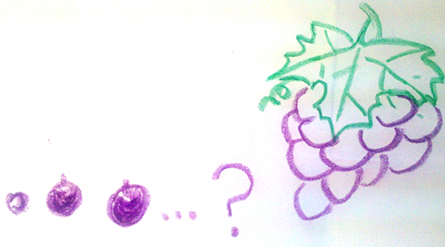
\includegraphics[scale=0.6]{img/grapes-1.eps}
  \caption{Always picking the smallest grape.} 
  \label{fig:eat-grapes}
\end{figure}

Based on this idea, the algorithm of selection sort can be directly
described as the following. 

In order to sort a series of elements:

\begin{itemize}
\item The trivial case, if the series is empty, then we are done, the result is also empty;
\item Otherwise, we find the smallest element, and append it to the tail of the result;
\end{itemize}

Note that this algorithm sorts the elements in increase order; It's easy to sort in decrease
order by picking the biggest element intead; We'll introduce about passing a comparator as
parameter later on.

This description can be formalized to a equation.

\be
sort(A) =  \left \{
  \begin{array}
  {r@{\quad:\quad}l}
  \Phi & A = \Phi \\
  \{ m \} \cup sort(A') & otherwise
  \end{array}
\right.  
\ee

Where $m$ is the minimum elenets among collection $A$, and $A'$ is all the rest elements
except $m$:

\[
\begin{array}{l}
m = min(A) \\
A' = A - \{ m \}
\end{array}
\]

We don't limit the data structure of the collection here. Typically, $A$ is array in imperative
environment, and list (singly linked-list particularly) in functional environment, and it can 
be even others as we introduced later.

The algorithm can also be given in imperative manner.

\begin{algorithmic}
\Function{Sort}{$A$}
  \State $X \gets \Phi$
  \While{$A \neq \Phi$}
    \State $x \gets$ \Call{Min}{$A$}
    \State $A \gets$ \Call{Del}{$A, x$}
    \State $X \gets$ \Call{Append}{$X, x$}
  \EndWhile
  \State \Return $X$
\EndFunction
\end{algorithmic}

Figure \ref{fig:sel-sort} dipicts the process of this algorithm.

\begin{figure}[htbp]
  \centering
  \includegraphics[scale=0.8]{img/sel-sort.ps}
  \caption{The left part is sorted data, continuously pick the minimum element in the rest and append it to the ressult.} 
  \label{fig:sel-sort}
\end{figure}

We just translate the very original idea of `eating grapes' line by line without
considering any expense of time and space cost. This realization store the result
in $X$, and when an selected element is appended to $X$, we delete the same element
from $A$. This indicates that we can change it to `in-place' sorting to reuse
the spaces in $A$.

The idea is to store the minimum element in the first cell in $A$ (we use term `cell' if
$A$ is array, and say `node' if $A$ is list); then store the second minimum element
in next cell, then third cell, ... 

One solution to realize this sorting strategy is swapping. When we select the $i$-th 
minimum element, we swap it with the element in the $i$-th cell:

\begin{algorithmic}
\Function{Sort}{$A$}
  \For{$i \gets 1$ to $|A|$}
    \State $m \gets$ \Call{Min}{$A[i...]$}
    \State \textproc{Exchange} $A[i] \leftrightarrow m$
  \EndFor
\EndFunction
\end{algorithmic}

Denote $A = \{a_1, a_2, ..., a_N\}$. At any time, when we process the $i$-th element, 
all elements before $i$, as $\{a_1, a_2, ..., a_{i_1}\}$ have already been sorted. 
We locate the minimum element among the $\{a_i, a_{i+1}, ..., a_N\}$, and exchange it
with $a_i$, so that the $i$-th cell contains the right value. The process is repeatedly
executed till we arrived at the last element. 

This idea can be illustrated by figure \ref{fig:in-place-sort}.

\begin{figure}[htbp]
  \centering
  \includegraphics[scale=0.8]{img/in-place-sort.ps}
  \caption{The left part is sorted data, continuously pick the minimum element in the rest and put it to the right position.} 
  \label{fig:in-place-sort}
\end{figure}

% ================================================================
% Find the minimum
% ================================================================
\section{Finding the minimum}
\index{selection sort!minimum finding}

We haven't completely realized the selection sort, because we take the operation
of finding the minimum (maximum) element as a black box. It's a puzzle how does
a kid locate the biggest or the smallest grape. 
And this is an interesting topic for computer algorithms.

The easist but not so fast way to find the minimum in a collection is to perform
a scan. There are several ways to interprete this scan process. Consider that
we want to pick the biggest grape. We start from any grape, compare it with 
another one, and pick the bigger one; then we take a next grape and compare
it with the one we selected so far, pick the bigger one and go on the take-and-compare
process, until there is no any grape we haven't compared.

It's easy to get loss in real practice if we don't mark which grape has been 
compared. There are two ways to to solve this problem, which are suitable for
different data-structures respectively.

\subsection{Labeling}
Method 1 is to label each grape with a number: $\{1, 2, ..., N\}$, and we systematically
perform the compare in the order of this sequence of labels. That we first 
compare grape number 1 and grape number 2, pick the bigger one; then we take grape
number 3, and do the comparation, ... We repeat this process until arrived at
grape number $N$. This is quite suitable for elements stored in an array.

\begin{algorithmic}
\Function{Min}{$A$}
  \State $m \gets A[1]$
  \For{$i \gets 2$ to $|A|$}
    \If{$A[i] < m$}
      \State $m \gets A[i]$
    \EndIf
  \EndFor
  \State \Return $m$
\EndFunction
\end{algorithmic}

With \textproc{Min} defined, we can complete the basic version of selection sort
(or naive version without any optimization in terms of time and space). 

However, this algorithm returns the value of the minimum element instead of its
location (or the label of the grape), which need a bit tweaking for the in-place version.
Some languages such as ISO C++, support returning the reference as result, so that the
swap can be achieved directly as below.

\lstset{language=C++}
\begin{lstlisting}
template<typename T>
T& min(T* from, T* to) {
    T* m;
    for (m = from++; from != to; ++from)
        if (*from < *m)
            m = from;
    return *m;
}

template<typename T>
void ssort(T* xs, int n) {
    int i;
    for (i = 0; i < n; ++i)
        std::swap(xs[i], min(xs+i, xs+n));
}
\end{lstlisting}

In environments without reference semantics, the solution is to return the location
of the minimum element instead of the value:

\begin{algorithmic}
\Function{Min-At}{$A$}
  \State $m \gets$ \Call{First-Index}{$A$}
  \For{$i \gets m + 1 $ to $|A|$}
    \If{$A[i] < A[m]$}
      \State $m \gets i$
    \EndIf
  \EndFor
  \State \Return $m$
\EndFunction
\end{algorithmic}

Note that since we pass $A[i...]$ to \textproc{Min-At} as the argument, we assume the first
element $A[i]$ as the smallest one, and examine all elements $A[i+1], A[i+2], ...$ one by one.
Function \textproc{First-Index}() is used to retrieve $i$ from the input parameter.

The following Python example program, for example, completes the basic in-place
selection sort algorithm based on this idea. It explicitly passes the range information
to the function of finding the minimum location.

\lstset{language=Python}
\begin{lstlisting}
def ssort(xs):
    n = len(xs)
    for i in range(n):
        m = min_at(xs, i, n)
        (xs[i], xs[m]) = (xs[m], xs[i])
    return xs

def min_at(xs, i, n):
    m = i;
    for j in range(i+1, n):
        if xs[j] < xs[m]:
            m = j
    return m
\end{lstlisting}

\subsection{Groupping}
Another method is to group all grapes in two parts: the group we have examined, and rest we
haven't. We denote these two groups as $A$ and $B$; All the elements (grapes) as $L$. 
At the beginning, we haven't examine any grapes at all, thus $A$ is empty ($\Phi$), and
$B$ contains all grapes. We can select arbitary two grapes from $B$, compare them, and 
put the loser (the smaller one for example) to $A$. After that, we repeat this process
by continously picking arbitrary grapes from $B$, and compare with the winner of the
previous time until $B$ becomes empty. At this time being, the final winner is the
minimum element. And $A$ turns to be $L - \{min(L)\}$, which can be used for the next
time minimum finding.

There is an invariant of this method, that at any time, we have $L = A \cup \{m\} \cup B$,
where $m$ is the winner so far we hold.

This approach doesn't need the collection of grapes being indexed (as being labeled
in method 1). It's suitable for any traversable data structures, including linked-list
etc. This method can be formalized as the below auxiliary function.

\be
min'(A, m, B) =  \left \{
  \begin{array}
  {r@{\quad:\quad}l}
  (m, A) & B = \Phi \\
  min'(A \cup \{m\}, b_1, B') & b_1 < m \\
  min'(A \cup \{b_1\}, m, B') & otherwise
  \end{array}
\right.  
\ee

In order to pick the minimum element, we call this auxiliar function by passing
an empty $A$, and use an arbitrary element (for instance, the first one) 
to initialize $m$:

\be
extractMin(L) = min'(\Phi, l_1, L')
\ee

Where $L'$ is all elements in $L$ except for the first one $l_1$. The algorithm
$extractMin)$ doesn't not only find the minimum elment, but also returns the
updated collection which doesn't contains the minimum. Summarize this minimum
extracting algorithm up to the basic selection sort defintion, we can create
a complete functional sorting program.

\lstset{language=Haskell}
\begin{lstlisting}
sort [] = []
sort xs = x : sort xs' where
  (x, xs') = extractMin xs
  
extractMin (x:xs) = min' [] x xs where
  min' ys m [] = (m, ys)
  min' ys m (x:xs) = if m < x then min' (x:ys) m xs else min' (m:ys) x xs
\end{lstlisting}

The first line handles the trivial edge case that the sorting result for empty
list is obvious empty; The second clause ensures that, there is at least one
element, that's why the \verb|extractMin| function needn't other pattern-matching.

One may think the second clause of \verb|min'| function should be written like below:

\begin{lstlisting}
min' ys m (x:xs) = if m < x then min' ys ++ [x] m xs 
                            else min' ys ++ [m] x xs
\end{lstlisting}

Or it will produce the updated list in reverse order. However, it's neccessary to
use `cons' instead of appending here. This is because appending is linear operation
which is proportion to the length of part $A$, while `cons' is constant $O(1)$ time
operation. Actually, we needn't keep the relative order of the list to be sorted,
as it will be re-arrnaged anyway during sorting. 

It's quite possible to keep the relative order during sorting, while ensure the
performance of finding the minimum element not degrade to quadratic. The following
equation defines a solution.

\be
extractMin(L) = \left \{
  \begin{array}
  {r@{\quad:\quad}l}
  (l_1, \Phi) & |L| = 1 \\
  (l_1, L') & l_1 < m, (m, L'') = extractMin(L') \\
  (m, {l_1} \cup L'') & otherwise
  \end{array}
\right.  
\ee

If $L$ is a singleton, the minimum is the only element it contains. Otherwise,
denote $l_1$ as the first element in $L$, and $L'$ contains the rest elements except
for $l_1$, that $L' = \{ l_2, l_3, ...\}$. The algorithm recursively finding
the minimum element in $L'$, which yields the intermediate result as $(m, L'')$,
that $m$ is the minimum element in $L'$, and $L''$ contains all rest elements
except for $m$. Comparing $l_1$ with $m$, we can determine which of them are
the final minimum result.

The following Haskell program implements this version of selection sort.

\begin{lstlisting}
sort [] = []
sort xs = x : sort xs' where
  (x, xs') = extractMin xs

extractMin [x] = (x, [])
extractMin (x:xs) = if x < m then (x, xs) else (m, x:xs') where
  (m, xs') = extractMin xs
\end{lstlisting}

Note that only `cons' operation is used, we needn't appending at all because
the algorithm actually examines the list from right to left. However, it's not
free, as this program need book-keeping the context (via call stack typically).
The relative order is ensured by the nature of recursion. Please refer
to the appendix about tail recursion call for detailed discussion.

\subsection{performance of the basic selection sorting}

Both the labeling method, and the grouping method need examine all the elements to
pick the minimum in every round; and we totally pick up minimum element $N$ times.
Thus the performance is around $N + (N-1) + (N-2) + ... + 1$ which is $\frac{N(N+1)}{2}$.
Selection sort is a quadratic algorithm bound to $O(N^2)$ time.

Compare to the insertion sort, which we introduced previously, selection sort
performs same in its bese case, worst case and average case. While insertion
sort performs well in best case (that the list has been reverse ordered, and it is stored
in linked-list) as $O(N)$, and the worst performance is $O(N^2)$. 

In the next sections, we'll examine, why selection sort performs poor, and try
to improve it step by step. 

\begin{Exercise}

\begin{itemize}
\item Implement the basic imperative selection sort algorithm (the none in-place version)
in your favorite programming language. Compare it with the in-place version, and analyze
the time and space effectiveness.
\end{itemize}

\end{Exercise}

% ================================================================
% Improvement 1
% ================================================================

\section{Minor Improvement}

\subsection{Parameterize the comparator}
Before any improvement in terms of performance, let's made the selection sort
algorithm general enough to handle different sorting criteria.

We've seen two opposite examples so far, that one may need sort the elements
in ascending order or descending order. For the former case, we need 
repleatedly finding the minimum, while for the later, we need find the maximum
instead. They are just two special cases. In real world practice, one 
may want to sort things in varies criteria, e.g. in terms of size, weight,
age, ... 

One solution to handle them all is to passing the criteria as a compare function
to the basic selection sort algorithms. For example:

\be
sort(c, L) = \left \{
  \begin{array}
  {r@{\quad:\quad}l}
  \Phi & L = \Phi \\
  {m} \cup sort(c, L'') & otherwise, (m, L'') = extract(c, L')
  \end{array}
\right.  
\ee

And the algorithm $extract(c, L)$ is defined as below.

\be
extract(c, L) = \left \{
  \begin{array}
  {r@{\quad:\quad}l}
  (l_1, \Phi) & |L| = 1 \\
  (l_1, L') & c(l_1, m), (m, L'') = extract(c, L') \\
  (m, \{l_1\} \cup L'') & \lnot c(l_1, m)
  \end{array}
\right.  
\ee

Where $c$ is a comparator function, it takes two elements, compare them and
returns the result of which one is preceding of the other. 
Passing `less than' operator $(<)$ turns this algorithm to be the version
we introduced in previous section.

Some environment require to pass the total ordering comparator, which 
returns result among `less than', 'equal', and 'greater than'. We needn't
such strong condition here, that $c$ only test if `less than' is satisfied.
However, as the minimum requirement, the comparator should meet the
strict weak ordering as following \cite{wiki-sweak-order}:

\begin{itemize}
\item Irreflexivity, for all $x$, it's not the case that $x < x$;
\item Asymmetric, For all $x$ and $y$, if $x < y$, then it's not the case $y < x$;
\item Transtivity, For all $x$, $y$, and $z$, if $x < y$, and $y < z$, then $x < z$;
\end{itemize}

The following Scheme/Lisp program translates this generic selection sorting algorithm.
The reason why we choose Scheme/Lisp here is because the lexical scope can simplify
the needs to pass the `less than' comparator for every function calls.

\lstset{language=Lisp}
\begin{lstlisting}
(define (sel-sort-by ltp? lst)
  (define (ssort lst)
    (if (null? lst)
        lst
        (let ((p (extract-min lst)))
          (cons (car p) (ssort (cdr p))))))
  (define (extract-min lst)
    (if (null? (cdr lst))
        lst
        (let ((p (extract-min (cdr lst))))
          (if (ltp? (car lst) (car p))
              lst
              (cons (car p) (cons (car lst) (cdr p)))))))
  (ssort lst))
\end{lstlisting}

Note that, both \verb|ssort| and \verb|extract-min| are inner functions, so that the
`less than' comparator \verb|lt?| is available to them. Passing `$<$' to this function
yields the normal sorting in ascending order:

\lstset{language=Lisp}
\begin{lstlisting}
(sel-sort-by < '(3 1 2 4 5 10 9))
;Value 16: (1 2 3 4 5 9 10)
\end{lstlisting}

It's possible to pass varies of comparator to imperative selection sort as well. This
is left as an exercise to the reader.

For the sake of brevity, we only consider sorting elements in ascending order in
the rest of this chapter. And we'll not pass comparator as a parameter unless it's
neccessary.

\subsection{Trivial fine tune}

The basic in-place imperative selection sorting algorithm iterates all elements, and picking the
minimum element by traversing as well. It can be written in a compact way, that we 
inline the minimum finding part as an inner loop.

\begin{algorithmic}
\Procedure{Sort}{$A$}
  \For{ $i \gets 1$ to $|A|$}
    \State $m \gets i$
    \For{$j \gets i+1$ to $|A|$}
      \If{$A[i] < A[m]$}
        \State $m \gets i$
      \EndIf
    \EndFor
    \State \textproc{Exchange} $A[i] \leftrightarrow A[m]$
  \EndFor
\EndProcedure
\end{algorithmic}

Observe that, when we are sorting $N$ elements, after the first $N-1$ minimum ones are selected,
the left only one, is definitely the $N$-th big element, so that we need NOT find the 
minimum if there is only one element in the list. This indicates that the outter loop can
iterate to $N-1$ instead of $N$.

Another place we can fine tuned, is that we needn't swap the elements if the $i$-th minimum one
is just $A[i]$. The algorithm can be modified accordingly as below:

\begin{algorithmic}
\Procedure{Sort}{$A$}
  \For{ $i \gets 1$ to $|A|-1$}
    \State $m \gets i$
    \For{$j \gets i+1$ to $|A|$}
      \If{$A[i] < A[m]$}
        \State $m \gets i$
      \EndIf
    \EndFor
    \If{$m \neq i$}
      \State \textproc{Exchange} $A[i] \leftrightarrow A[m]$
    \EndIf
  \EndFor
\EndProcedure
\end{algorithmic}

Definitely, these modifications won't affects the performance in terms of big-O.

\subsection{Cock-tail sort}

Knuth gave an alternative realization of selection sort in \cite{TAOCP}. Instead of selecting the
minimum each time, we can select the maximum element, and put it to the last position. This method
can be illustrated by the following algorithm.

\begin{algorithmic}
\Procedure{Sort'}{$A$}
  \For{ $i \gets |A|$ down-to $2$}
    \State $m \gets i$
    \For{$j \gets 1$ to $i-1$}
      \If{$A[m] < A[i]$}
        \State $m \gets i$
      \EndIf
    \EndFor
    \State \textproc{Exchange} $A[i] \leftrightarrow A[m]$
  \EndFor
\EndProcedure
\end{algorithmic}

As shown in figure \ref{fig:knuth-ssort}, at any time, the elements on right most side
are sorted. The algorithm scans all unsorted ones, and locate the maximum. Then, put
it to the tail of the unsorted range by swapping.

\begin{figure}[htbp]
  \centering
  \includegraphics[scale=0.8]{img/knuth-ssort.ps}
  \caption{Select the maximum every time and put it to the end.}
  \label{fig:knuth-ssort}
\end{figure}

This version reveals the fact that, selecting the maximum element can sort the element in
ascending order as well. What's more, we can find both the minimum and the maximum elements
in one pass of traversing, putting the minimum at the first location, while putting the
maximum at the last position. This approach can speed up the sorting slightly (halve the
outter loop times).

\begin{algorithmic}
\Procedure{Sort}{$A$}
  \For{$i \gets 1 $ to $\lfloor \frac{|A|}{2} \rfloor$}
    \State $min \gets i$
    \State $max \gets |A| + 1 - i$
    \If{$A[max] < A[min]$}
      \State \textproc{Exchange} $A[min] \leftrightarrow A[max]$
    \EndIf
    \For{$j \gets i + 1$ to $|A| - i$}
      \If{$A[j] < A[min]$}
        \State $min \gets j$
      \EndIf
      \If{$A[max] < A[j]$}
        \State $max \gets j$
      \EndIf
    \EndFor
    \State \textproc{Exchange} $A[i] \leftrightarrow A[min]$
    \State \textproc{Exchange} $A[|A|+1-i] \leftrightarrow A[max]$
  \EndFor
\EndProcedure
\end{algorithmic}

This algorithm can be illustrated as in figure \ref{fig:cock-tail-sort}, at any time, the left most and right most
parts contains sorted elements so far. That the smaller sorted ones are on the left, while the bigger sorted ones
are on the right. The algorithm scans the unsorted ranges, located both the minimum and the maximum positions,
then put them to the head and the tail position of the unsorted ranges by swapping.

\begin{figure}[htbp]
  \centering
  \includegraphics[scale=0.7]{img/cock-tail-sort.ps}
  \caption{Select both the minimum and maximum in one pass, and put them to the proper positions.}
  \label{fig:cock-tail-sort}
\end{figure}

Note that the it's neccessary to swap the left most and right most elements before the inner loop if they are
not in correct order. This is because we scan the range excluding these two elements. Another method is to
initialize the first element of the unsorted range as both the maximum and minimum before the inner loop.
However, the since we need two swapping after the scan, so it possible that the first swapping moves
the maximum or the minimum from the position we just found, which leads the second swapping malfunctioned.
How to solve this problem is left as exercise to the reader.

The following Python example program implements this cock-tail sort algorithm.

\lstset{language=Python}
\begin{lstlisting}
def cocktail_sort(xs):
    n = len(xs)
    for i in range(n / 2):
        (mi, ma) = (i, n - 1 -i)
        if xs[ma] < xs[mi]:
            (xs[mi], xs[ma]) = (xs[ma], xs[mi])
        for j in range(i+1, n - 1 - i):
            if xs[j] < xs[mi]:
                mi = j
            if xs[ma] < xs[j]:
                ma = j
        (xs[i], xs[mi]) = (xs[mi], xs[i])
        (xs[n - 1 - i], xs[ma]) = (xs[ma], xs[n - 1 - i])
    return xs
\end{lstlisting}

It's possible to realize cock-tail sort in functional approach as well. An intuitive recursive description
can be give like this:

\begin{itemize}
  \item Trivial edge case: If the list is empty, or there is only one element in the list, the sorted result is obviously the origin list;
  \item Otherwise, we select the minimum and the maximum, put them in the head and tail position, then recursively sort the rest elements.
\end{itemize}

This algorithm description can be formalized by the following equation.

\be
sort(L) = \left \{
  \begin{array}
  {r@{\quad:\quad}l}
  L & |L| \leq 1 \\
  \{ l_{min} \} \cup sort(L'') \cup \{ l_{max} \} & otherwise
  \end{array}
\right.  
\ee

Where the minimum and the maximum are extracted from $L$ by a function $select(L)$.

\[
(l_{min}, L'', l_{max}) = select(L)
\]

Note that, the minimum is actually link to the front of the recursive sort result. Its semantic is a constant $O(1)$
time `cons' (refer to the appendix of this book for detail). While the maximum is appending to the tail. This
is typically a linear $O(N)$ time expensive operation. We'll optimize it later.

Function $select(L)$ scan the whole list to find both the minimum and the maximum. It can be defined as below:

\be
select(L) =  \left \{
  \begin{array}
  {r@{\quad:\quad}l}
  (min(l_1, l_2), max(l_1, l_2)) & L = \{ l_1, l_2\} \\
  (l_1, \{ l_{min}\} \cup L'', l_{max}) & l_1 < l_{min} \\
  (l_{min}, \{l_{max}\} \cup L'', l_1) & l_{max} < l_1 \\
  (l_{min}, \{l_1\} \cup L'', l_{max}) & otherwise
  \end{array}
\right.  
\ee

Where $(l_{min}, L'', l_{max}) = select(L')$ and $L'$ is the rest of the list except for the first element $l_1$.
If there are only two elements in the list, we pick the smaller as the minimum, and the bigger as the maximum.
After extact them, the list becomes empty. This is the trivial edge case; Otherwise, we take the first element
$l_1$ out, then recursively perform selection on the rest of the list. After that, we compare if $l_1$ is less
then the minimum or greater than the maximum candidates, so that we can finalize the result.

Note that for all the cases, there is no appending operation to form the result. However, since selection must
scan all the element to determin the minimum and the maximum, it is bound to $O(N)$ linear time.

The complete example Haskell program is given as the following.

\lstset{language=Haskell}
\begin{lstlisting}
csort [] = []
csort [x] = [x]
csort xs = mi : csort xs' ++ [ma] where
  (mi, xs', ma) = extractMinMax xs
  
extractMinMax [x, y] = (min x y, [], max x y)
extractMinMax (x:xs) | x < mi = (x, mi:xs', ma)
                     | ma < x = (mi, ma:xs', x)
                     | otherwise = (mi, x:xs', ma)
  where (mi, xs', ma) = extractMinMax xs
\end{lstlisting}

We mentioned that the appending operation is expensive in this intuitive version. It can be improved.
This can be achieved in two steps. The first step is to convert the cock-tail sort into tail-recursive
call. Denote the sorted small ones as $A$, and sorted big ones as $B$ in figure \ref{fig:cock-tail-sort}. 
We use $A$ and $B$ as accumulators. The new cock-tail sort is defined as the following.

\be
sort'(A, L, B) = \left \{
  \begin{array}
  {r@{\quad:\quad}l}
  A \cup L \cup B & L = Phi \lor |L| = 1 \\
  sort'(A \cup \{ l_{min}\}, L'', \{ l_{max}\} \cup B) & otherwise
  \end{array}
\right. 
\ee

Where $l_{min}$, $l_{max}$ and $L''$ are defined as same as before. And we start sorting by passing
empty $A$ and $B$: $sort(L) = sort'(\Phi, L, \Phi)$.

Besides the edge case, observing that the appending operation only happens on $A \cup {l_min}$; while
$l_{max}$ is only linked to the head of $B$. This appending occurs in every recursive call. To elemininate
it, we can store $A$ in reverse order as $\overleftarrow{A}$, so that $l_{max}$ can be `cons' to the
head instead of appending. Denote $cons(x, L) = \{x\} \cup L$ and $append(L, x) = L \cup \{x\}$, 
we have the below equation.

\be
\begin{array}{rl}
append(L, x) & = reverse(cons(x, reverse(L))) \\
             & = reverse(cons(x, \overleftarrow{L}))
\end{array}
\ee

Finally, we perform a reverse to turn $\overleftarrow{A}$ back to $A$. 
Based on this idea, the algorithm can be improved one more step as the following.

\be
sort'(A, L, B) = \left \{
  \begin{array}
  {r@{\quad:\quad}l}
  reverse(A) \cup B & L = \Phi \\
  reverse(\{l_1\} \cup A) \cup B & |L| = 1 \\
  sort'(\{l_{min}\} \cup A, L'', \{l_{max}\} \cup B)
  \end{array}
\right. 
\ee

This algorithm can be implemented by Haskell as below.

\lstset{language=Haskell}
\begin{lstlisting}
csort' xs = cocktail [] xs [] where
  cocktail as [] bs = reverse as ++ bs
  cocktail as [x] bs = reverse (x:as) ++ bs
  cocktail as xs bs = let (mi, xs', ma) = extractMinMax xs 
                      in cocktail (mi:as) xs' (ma:bs)  
\end{lstlisting}

\begin{Exercise}
  \begin{itemize}
    \item Realize the imperative basic selection sort algorithm, which can take a comparator as a parameter. Please try both dynamic typed langauge and static typed langauge. How to annotate the type of the comparator as general as possible in a static typed language? 
   \item Implement Knuth's version of selection sort in your favorite programming language.
   \item An alternative to realize cock-tail sort is to assume the $i$-th element both the minimum and the maximum, after the inner loop, the minimum and maximum are found, then we can swap the the minimum to the $i$-th position, and
the maximum to position $|A|+1-i$. Implement this solution in your favorite imperative language. Please note that
there are several special edge cases should be handled correctly:
    \begin{itemize}
      \item $A = \{max, min, ...\}$;
      \item $A = \{..., max, min\}$;
      \item $A = \{max, ..., min\}$.
    \end{itemize}
    Please don't refer to the example source code along with this chapter before you try to solve this problem.
  \end{itemize}
\end{Exercise}

% ================================================================
% Improvement 2
% ================================================================

\section{Major improvement}

Although cock-tail sort halves the numbers of loop, the performance is still bound to quadratic time.
It means that, the method we developed so far handles big data poorly compare to other divide and conquer
sorting solutions.

To improve selection based sort essentially, we must analyze where is the bottle-neck. In order to sort
the elements by comparason, we must examine all the elements for ordering. Thus the outter loop of selection
sort is neccessary. However, must it scan all the elements every time to select the minimum? Note that
when we pick the smallest one at the first time, we actually traverse the whole collection, so that
we know which ones are relative bigger, and which ones are relative small partially.

The problem is that, when we select the further minimum elements, instread of re-using the ordering information
we obtained previously, we drop them all, and blindly start a new traverse.

So the key point to improve selection based sort is to re-use the previous result. There are several approaches, 
we'll adopt an intuitive idea inspired by football match in this chapter.

\subsection{Tournament knock out}

The football world cup is held every four years. There are 32 teams from different continent 
play the final games. Before 1982, there were 16 teams compete for the tournament finals\cite{wiki-wc}.

For simplification purpse, let's go back to 1978 and imagine a way to determine the champion: 
In the first round, the teams
are grouped into 8 pairs to play the game; After that, there will be 8 winner, and 8 teams will
be out. Then in the second round, these 8 teams are groupped into 4 pairs. This time there
will be 4 winners after the second round of games; Then the top 4 teams are divided into 
2 pairs, so that there will be only two teams left for the final game. 

The chammpion is determined after the total 4 rounds of games. And there are actually $8+4+2+1 = 16$
games. Now we have the world cup champion, however, the world cup game won't finish at this stage,
we need to determine which is the silver medal team.

Readers may argue that isn't the team beat by the champion at the final game the second best?
This is true according to the real world cup rule. However, it isn't fair enough in some sense.

We often heard about the so called `group of death', Let's suppose that Brazile team is 
groupped with Deutch team at the very begining. Altough both teams are quite strong, one of
them must be knocked out. It's quite possible that even the team loss that game can beat
all the other teams except for the champion. Figure \ref{fig:tournament-tree-1} illustrates such
case.

\begin{figure}[htbp]
  \centering
  \includegraphics[scale=0.25]{img/tournament-tree-1.ps}
  \caption{The element 15 is knocked out in the first round.}
  \label{fig:tournament-tree-1}
\end{figure}

Imagine that every team has a number. The bigger the number, the stronger the team. Suppose
that the stronger team always beats the team with smaller number, although this is not true
in real world. But this simplification is fair enough for us to develop the tournament knock
out solution. This maximum number which represents the champion is 16. Definitely, team with
number 14 isn't the second best according to our rules. It should be 15, which is knocked
out at the first round of comparison.

The key quesion here is to find an effective way to locate the second maximum number in this
tournament tree. After that, what we need is to apply the same method to select the third,
the fourth, ..., to accomplish the selection based sort.

One idea is to assign the champion a very small number (for instance, $-\infty$), 
so that it won't be selected next time, and the second best one, becomes the new champion.
However, suppose there are $2^m$ teams for some natural number $m$, it still takes 
$2^{m_1} + 2^{m-2} + ... + 2 + 1 = 2^m$ times of comparison to determine the new 
champion. Which is as slow as the first time.

Actually, we needn't perform a bottom-up comparison at all since the tournament tree
stores plenty of ordering information. Observe that, the second best team must
be beaten by the champion at sometime, or it will be the final winner. So we
can track the path from the root of the tournament tree to the leaf of the
champion, examine all the teams along with this path to find the second best team.

In figure \ref{fig:tournament-tree-1}, this path is marked in gray color, the elements
to be examined are $\{14, 13, 7, 15\}$. Because the tournament tree is well balanced,
the length of this path, which is the height of the tree, is bound to $O(\lg N)$,
where $N$ is the number of the elements to be sorted.

\section{Short summary} 
In this chapter, we present the evolution process of insertion sort. Insertion
sort is well explained in most textbooks as the first sorting algorithm.
It has simple and straightforward idea, but the performance is quadratic.
Some textbooks stop here, but we want to show that there exist ways to improve
it by different point of view. We first try to save the comparison time
by using binary search, and then try to save the insertion operation by
changing the data structure to linked-list. Finally, we combine these
two ideas and evolute insertion sort to tree sort.

\begin{thebibliography}{99}

\bibitem{TAOCP}
Donald E. Knuth. ``The Art of Computer Programming, Volume 3: Sorting and Searching (2nd Edition)''. Addison-Wesley Professional; 2 edition (May 4, 1998) ISBN-10: 0201896850 ISBN-13: 978-0201896855

\bibitem{CLRS}
Thomas H. Cormen, Charles E. Leiserson, Ronald L. Rivest and Clifford Stein. 
``Introduction to Algorithms, Second Edition''. ISBN:0262032937. The MIT Press. 2001

\bibitem{wiki-sweak-order}
Wikipedia. ``Strict weak order''. http://en.wikipedia.org/wiki/Strict\_weak\_order

\bibitem{wiki-wc}
Wikipedia. ``FIFA world cup''. http://en.wikipedia.org/wiki/FIFA\_World\_Cup

\end{thebibliography}

\ifx\wholebook\relax\else
\end{document}
\fi
